\section{需求分析}

本程序要完成的功能为,将一段二进制序列转化为八进制的序列。
输入要求01序列,并且要以\#结束。
例如,
101010011010\#。
如果有必要,可以读入多个二进制串。
100110\#1010101\#。
我们对输入做出以下限制:
\begin{enumerate}
   \item 输入的串的长度不能超过$10^6$
   \item 输入的所有字符只能有0,1,\#
\end{enumerate}


在正常情况下,本程序输出一段8进制串。在有多个二进制串输入的情况下,
八进制串将按顺序输出。
以上面两个输入样例为例。


5232


46 125



\section{概要设计}
   main创建并初始化Solution结构,并且循环调用Solution中的读入和输出。


   Solution中保存了两个栈,一个用于放置二进制串,一个用于放置八进制串。
   栈中实现了push,pop,get\_top等栈的基本功能。
   Solution结构可以调用readBinary进行读入,调用writeOctal写入。
   再在Solution中实现一个可以将二进制数转化为八进制的中间函数。

\section{详细设计}

\begin{figure}[H]
   \centering
   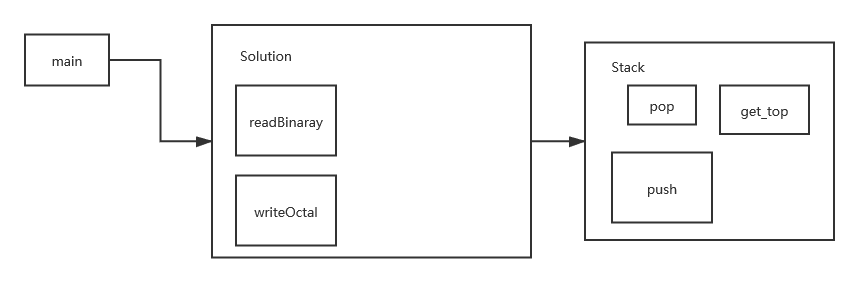
\includegraphics[width=0.5\textwidth]{images/process.png}
   \caption{函数调用关系图}
\end{figure}

\newpage

\begin{algorithm}[htb] 
   \caption{ Solution结构定义 } 
   \label{alg:Framwork} 
   \begin{algorithmic}[1]
      \Require 输入二进制串
      \Ensure 输出八进制串
      
      \State 读入二进制串
      \Function {readBinary}{void}
         \State 读入字符a
         \While {a不是\#也不是EOF}
            \If {a是错误字符}
               \State 输出错误
            \EndIf
            \State 将a加入到栈binary中
         \EndWhile
      \EndFunction \\

      \State 输出八进制串
      \Function {writeOctal}{void}
         \While{binary栈中不为空}
            \State temp = 在栈中取三个bit转化为八进制数
            \State 将temp加入到Octal中
         \EndWhile
      \EndFunction
   \end{algorithmic} 
\end{algorithm}

\section{调试分析报告}
   使用栈数据结构完成这个任务较为平凡。值得一提的是我们完成了对栈的封装,使得他可以在其他实验中复用。


   在使用线性数据结构的操作下,算法复杂度几乎已经达到了下界,即$O(N)$。
   但是空间复杂度上面还有许多可以优化的地方。我们人为定义的数据上限为$10^6$。但是显然,
   在大多数情况下用户使用的空间会远远低于这个上界。所以一次申请$10^6$显然是过度浪费内存的。


   所以我们将栈的数据存储到一个叫做Vector的动态数组中,这个数组开始时数据边界为$10^2$级别。
   在使用过程中,这个数组会自动调用$resize()$扩大边界。我们设一个系数$k$,每次$resize()$后的边界为原来的$k$倍。
   接下来我们将测试不同$k$下由$resize$造成的浪费。



% Please add the following required packages to your document preamble:
% \usepackage{booktabs}
% \usepackage{longtable}
% Note: It may be necessary to compile the document several times to get a multi-page table to line up properly
\begin{longtable}[c]{@{}lllll@{}}
   \toprule
   N   & $10^4$ & $10^5$ & $10^6$ &  \\* \midrule
   \endfirsthead
   %
   \endhead
   %
   \bottomrule
   \endfoot
   %
   \endlastfoot
   %
   1.6 & 29634  & 121688 & 121688 &  \\
   2.0 & 32704  & 65472  & 65472  &  \\
   2.4 & 20807  & 120056 & 120056 &  \\* \bottomrule
   \end{longtable}


   观察发现,在$k=1.6$与$k=2.4$时,数据表现较为极端,而$k=2.0$时较为平稳,所以我们选择$k=2.0$作为我们的vector的resize系数。


\section{用户使用说明}
   用户可以使用IDE或者手动编译源代码stack.cpp,获得可执行文件。
      
   笔者使用的gcc版本为8.1.0
   运行可执行文件后,用户可以选择文件输入或者交互式输入。
   在文件输入下输出将会从定向到output.in。
   结束程序可以输入EOF

\section{测试结果}
   用于测试的样例分为两部分,一部分为功能性样例,用于测试程序的正确性。另外一个为极端样例,用generator.cpp编译得到的可执行文件生成,
   用于测试程序的性能。


   我们构造的功能测试样例为


   101010011010 -> 5232


   100110\#1010101\# -> 46 125


   在程序中输入显示结果与手算相符




